\chapter{Sequential Building Blocks}
\graphicspath{ {./chapter06/FigWork} }
%%%%%%%%%%%%%%%%%%%%%%%%%%%%%%%%%%%%%%%%%%%%%%%%%%%%
%% Here are the helpful stuff
%%%%%%%%%%%%%%%%%%%%%%%%%%%%%%%%%%%%%%%%%%%%%%%%%%%%
\section{Helpful Stuff}

Here are the devices introduced in this chapter.

\begin{tabular}{|l|p{3.5in}|} \hline
    Nomenclature:  & N-bit register                               \\ \hline
    Data Input:    & N-bits vector $D=d_{N-1} \ldots d_1 d_0$.  \\ \hline
    Data Output:   & N-bit vector $Q=q_{N-1} \ldots q_1 q_0$    \\ \hline
    Control:       & 1-bit $c$                              \\ \hline
    Status:        & none                             \\ \hline
    Others:        & 1-bit edge-sensitive clock.  1-bit asynchronous
    active low reset.                        \\ \hline
    Behavior:      &
    \begin{tabular}{c|c|c|c||c||c}
        reset & clk          & C & D & $Q^+$ & comment \\ \hline
        0     & x            & x & x & $0$   & reset   \\ \hline
        1     & 0,1,falling  & x & x & $Q$   & hold  \\ \hline
        1     & rising       & 0 & x & $Q$   &  hold \\ \hline
        1     & rising       & 1 & D & D     &  load \\
    \end{tabular} \\ \hline
\end{tabular}

\begin{tabular}{|l|p{3.5in}|} \hline
    Nomenclature:  & N-bit shift register with parallel load     \\ \hline
    Data Input:    & N-bits vector $D=d_{N-1} \ldots d_1 d_0$.          \\ \hline
    Data Output:   & N-bit vector $Q=q_{N-1} \ldots q_1 q_0$    \\ \hline
    Control:       & 2-bits $c=c_1 c_0$              \\ \hline
    Status:        & none                                   \\ \hline
    Others:        & 1-bit edge-sensitive clock.  1-bit asynchronous
    active low reset.                       \\ \hline
    Behavior:      &
    \begin{tabular}{c|c|c|c||c||c}
        reset & clk          & C  & D & $Q^+$ & comment \\ \hline
        0     & x            & xx & x & $0$   & reset   \\ \hline
        1     & 0,1,falling  & xx & x & $Q$   & hold  \\ \hline
        1     & rising       & 00 & x & $Q$   &  hold \\ \hline
        1     & rising       & 01 & x & $Q>>1$   &  shift right \\ \hline
        1     & rising       & 10 & x & $Q<<1$   &  shift left \\ \hline
        1     & rising       & 11 & x & D     &  load \\
    \end{tabular} \\ \hline
\end{tabular}

\begin{tabular}{|l|p{4.5in}|} \hline
    Nomenclature:  & N-bit counter with parallel load                  \\ \hline
    Data Input:    & N-bits vector $D=d_{N-1} \ldots d_1 d_0$.          \\ \hline
    Data Output:   & N-bit vector $Q=q_{N-1} \ldots q_1 q_0$    \\ \hline
    Control:       & 2-bits $c=c_1 c_0$              \\ \hline
    Status:        & none                                   \\ \hline
    Others:        & 1-bit edge-sensitive clock.  1-bit asynchronous
    active low reset.                       \\ \hline
    Behavior:      &

    \begin{tabular}{c|c|c|c||c||c}
        reset & clk          & C  & D   & $Q^+$  & comment     \\ \hline
        0     & x            & xx & x   & $0$    & reset       \\ \hline
        1     & 0,1,falling  & xx & x   & $Q$    & hold        \\ \hline
        1     & rising       & 00 & x   & $Q$    & hold        \\ \hline
        1     & rising       & 01 & x   & $D$    & count up    \\ \hline
        1     & rising       & 10 & D   & $D$    & count up    \\ \hline
        1     & rising       & 11 & x   & $D$    & load        \\
    \end{tabular}    \\  \hline
\end{tabular}

\begin{tabular}{|l|p{4.5in}|} \hline
    Nomenclature:  & three state buffer                   \\ \hline
    Data Input:    & 1-bit X.          \\ \hline
    Data Output:   & 1-bit Y    \\ \hline
    Control:       & 1-bit $c$              \\ \hline
    Status:        & none                                   \\ \hline
    Others:        & none                 \\ \hline
    Behavior:      & Output equals input when $C=1$ otherwise
    output disconnected from input.    \\ \hline
\end{tabular}

\begin{tabular}{|l|p{4.5in}|} \hline
    Nomenclature:  & NxM RAM (random access memory)    \\ \hline
    Data Input:    &  M-bit vector $D=d_{M-1} \ldots d_1 d_0$
    $log_2(N)$-bit address $A=a_{log_2(N)-1} \ldots a_1 a_0$ \\ \hline
    Data Output:   & M-bit vector $D=d_{M-1} \ldots d_1 d_0$     \\ \hline
    Control:       & 1-bit CS (chip select), RE (Read enable),
    WE (write enable)             \\ \hline
    Status:        & none                                   \\ \hline
    Others:        & none                 \\ \hline
    Behavior:      &
    \begin{tabular}{c|c|c|c||c|l}
        A & CS  & RE   & WE & D  & Note   \\ \hline
        x & 0   & x    & x  & Z  & RAM deactivated      \\ \hline
        x & 1   & 0    & 0  & Z  & RAM deactivated \\ \hline
        A & 1   & 0    & 1  & D  & RAM[A] = D (write) \\ \hline
        A & 1   & 1    & 0  & RAM[A]   & D = RAM[A] (read)  \\
    \end{tabular} \\ \hline
\end{tabular}

\begin{tabular}{c|c|c}
    & Left            & Right            \\ \hline
    Arithmetic    & $x_2 x_1 x_0 0$        & $x_3 x_3 x_2 x_1$ \\ \hline
    Circular    & $x_2 x_1 x_0 x_3$    & $x_0 x_3 x_2 x_1$ \\ \hline
    Logical     & $x_2 x_1 x_0 0$        & $0   x_3 x_2 x_1$   \\
\end{tabular}

%%%%%%%%%%%%%%%%%%%%%%%%%%%%%%%%%%%%%%%%%%%%%%%%%%%%
%% Here are terms that the students define
%%%%%%%%%%%%%%%%%%%%%%%%%%%%%%%%%%%%%%%%%%%%%%%%%%%%

%%%%%%%%%%%%%%%%%%%%%%%%%%%%%%%%%%%%%%%%%%%%%%%%%%%%
%% Here are the problems
%%%%%%%%%%%%%%%%%%%%%%%%%%%%%%%%%%%%%%%%%%%%%%%%%%%%
\section{Problems}
\begin{description}

    \item[Plot] Complete the timing diagram for the register.
        You may assume that Q is initially 0.

        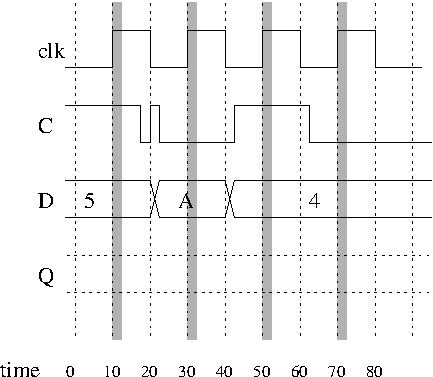
\includegraphics{OneBitTime}

    \item[Plot] Let
        $Q_{sr}$ is the output of a logical shift register
        (assume that 0 is shifted into the vacated bit position.
            Let $Q_{cnt}$ is the output of a counter.

            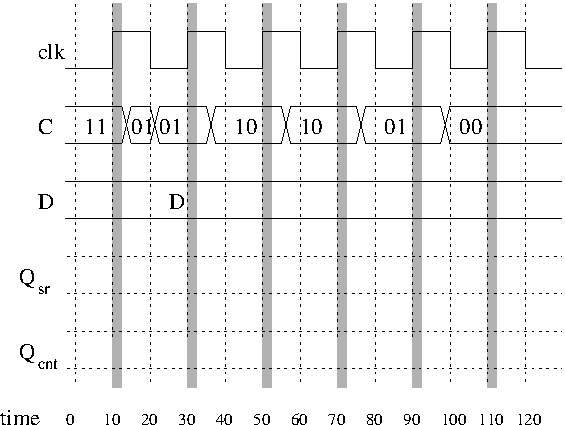
\includegraphics{TwoBitTime}

        \item[Label the mux inputs.]
            Make the resulting circuit operate according to the
            truth table shows at left.

            \begin{tabular}{ll}
                \begin{tabular}{c|c|c|c||c||c}
                    reset & clk          & C  & D   & $Q^+$  & comment     \\ \hline
                    0     & x            & xx & x   & $0$    & reset       \\ \hline
                    1     & 0,1,falling  & xx & x   & $Q$    & hold        \\ \hline
                    1     & rising       & 00 & x   & $Q$    & hold        \\ \hline
                    1     & rising       & 01 & x   & 0      & clear       \\ \hline
                    1     & rising       & 10 & D   & $Q+1$  & count up    \\ \hline
                    1     & rising       & 11 & x   & $D$    & load        \\
                \end{tabular}
                &
                \scalebox{0.5}{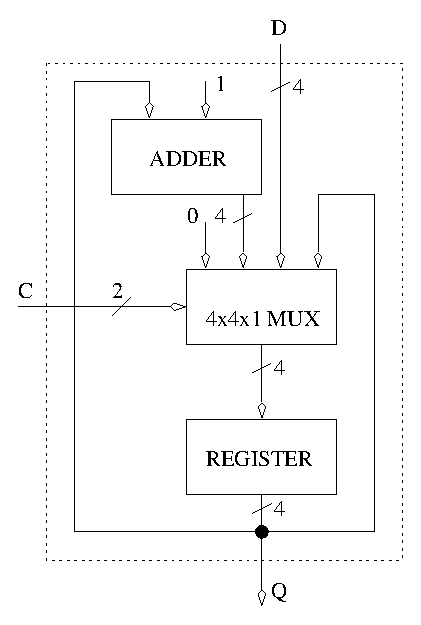
\includegraphics{Wire}}
            \end{tabular}

            \vspace{1cm}

        \item[Complete the timing diagram.]  Note any changes in
            the RAMs content.

            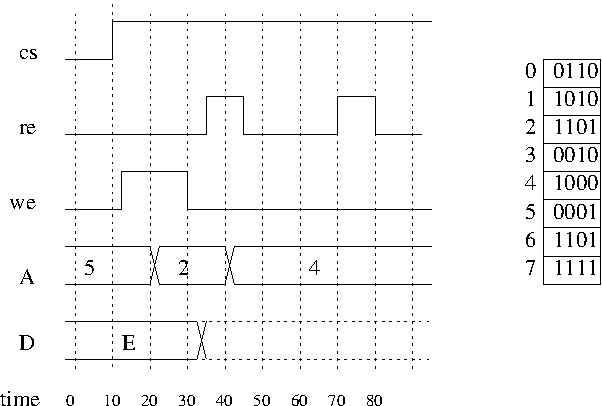
\includegraphics{RAMTime}

            \pagebreak

        \item[Complete the timing diagram.]  Use the counter control table
            from page 128.  Assume that c1=L and c0=L'.

            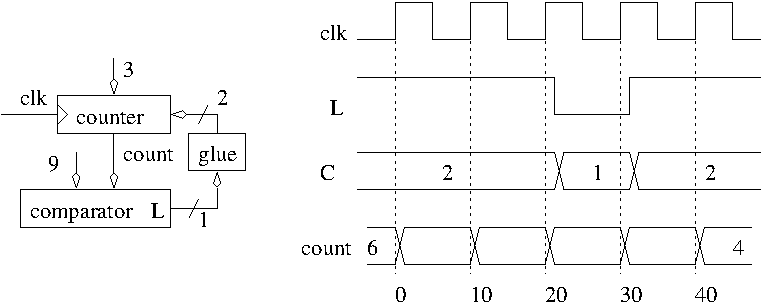
\includegraphics{work1}

        \item[Complete the timing diagram.]  Put "u" in spaces where the output
            is undefined.

            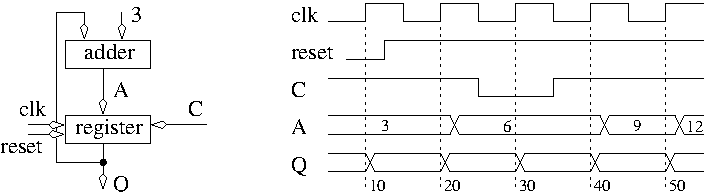
\includegraphics{work2}

        \item[Complete the timing diagram.]  Put "u' in spaces where the output
            is undefined.

            \scalebox{0.7}{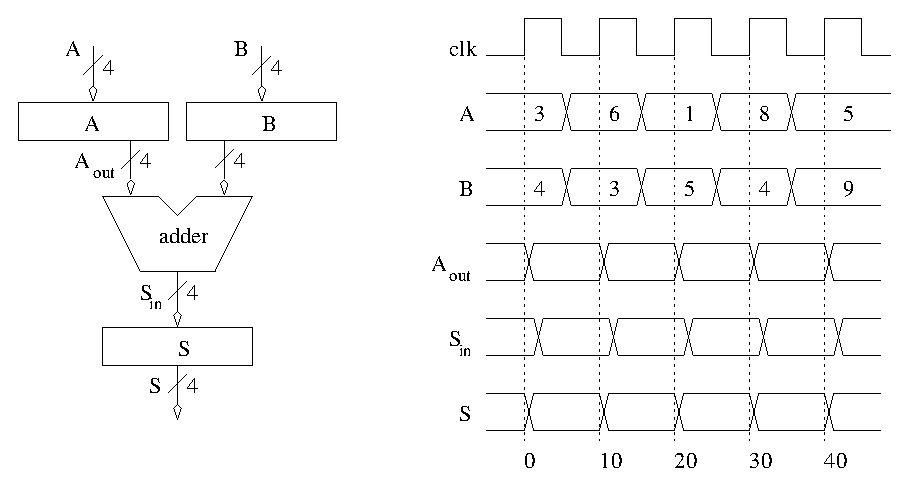
\includegraphics{work3}}

            \pagebreak
            %% Insert a simple circuit (counter like) with feedback
            %%        register
            %%        adder
            %%        compare + mux
        \item[Complete the timing diagram for the following circuit.]
            Note the labels of the signals.

            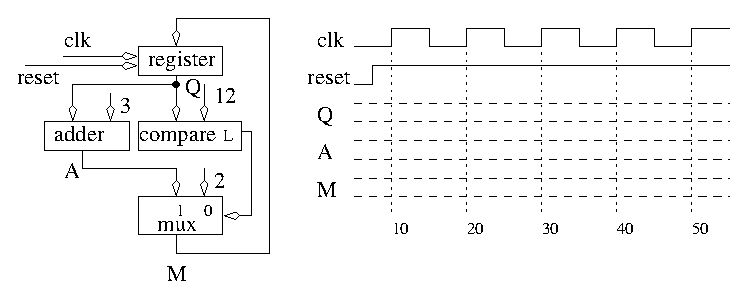
\includegraphics{BBBtiming1}

            %% Insert a complex circuit (counter like) with feedback
            %%        register
            %%        adder
            %%        register
            %%        compare + mux
        \item[Complete the timing diagram for the following circuit.]
            Note the labels of the signals.

            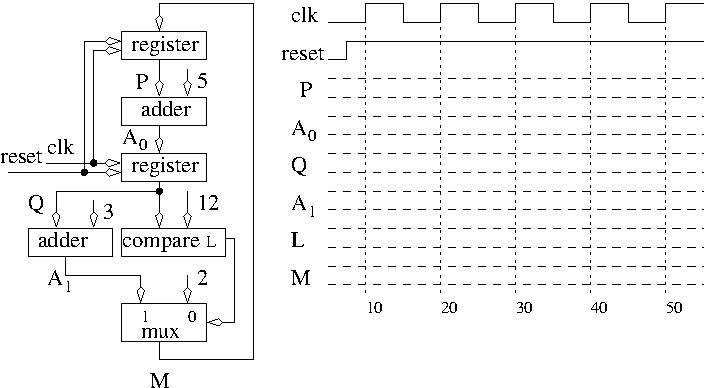
\includegraphics{BBBtiming2}

    \end{description}
